\documentclass[tikz,border=10pt]{standalone}
\usepackage{tikz}
\usetikzlibrary{arrows.meta, positioning, calc, matrix}

\begin{document}
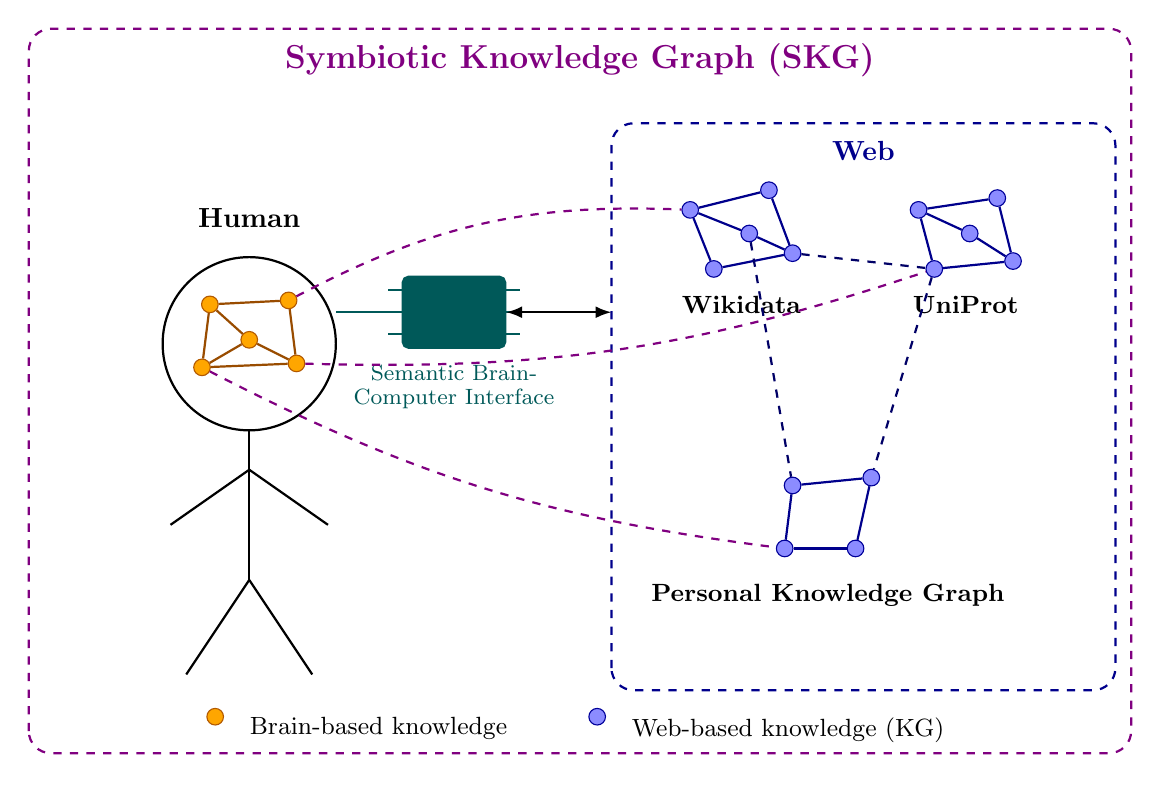
\begin{tikzpicture}[
  brainnode/.style={circle, draw=orange!70!black, fill=orange!70!yellow, minimum size=6pt, inner sep=0pt},
  webnode/.style={circle, draw=blue!60!black, fill=blue!45!white, minimum size=6pt, inner sep=0pt},
  brainedge/.style={thick, orange!60!black},
  weblink/.style={thick, blue!55!black},
  interlink/.style={thick, blue!40!black, dashed},
  symlink/.style={thick, violet, dashed},
  every node/.style={font=\small},
]

%% ============ OUTER SKG BOUNDARY ============
\draw[dashed, thick, violet, rounded corners=8pt] (-2.8,-4.6) rectangle (11.2,4.6);
\node[violet, font=\large\bfseries] at (4.2,4.2) {Symbiotic Knowledge Graph (SKG)};

%% ============ STICK FIGURE ============
% head
\draw[thick] (0,0.6) circle (1.1);
% body
\draw[thick] (0,-0.5) -- (0,-2.4);
% arms
\draw[thick] (0,-1.0) -- (-1.0,-1.7);
\draw[thick] (0,-1.0) -- (1.0,-1.7);
% legs
\draw[thick] (0,-2.4) -- (-0.8,-3.6);
\draw[thick] (0,-2.4) -- (0.8,-3.6);

\node[font=\bfseries] at (0,2.2) {Human};

%% ---- brain-based KG, drawn inside the head ----
\node[brainnode] (b1) at (-0.5,1.1)  {};
\node[brainnode] (b2) at (0.5,1.15)  {};
\node[brainnode] (b3) at (0.6,0.35)  {};
\node[brainnode] (b4) at (-0.6,0.3)  {};
\node[brainnode] (b5) at (0,0.65)    {};

\draw[brainedge] (b1)--(b2);
\draw[brainedge] (b1)--(b4);
\draw[brainedge] (b2)--(b3);
\draw[brainedge] (b3)--(b4);
\draw[brainedge] (b1)--(b5);
\draw[brainedge] (b3)--(b5);
\draw[brainedge] (b4)--(b5);

%% ============ SBCI CHIP ============
\node[draw, fill=teal!12, thick, minimum width=1.3cm, minimum height=0.9cm,
      rounded corners=2pt, teal!70!black] (chip) at (2.6,1.0) {\textbf{SBCI}};

% little chip "pins"
\foreach \y in {-0.28,0,0.28}{
  \draw[teal!70!black, thick] ($(chip.west)+(0,\y)$) -- ++(-0.18,0);
}
\foreach \y in {-0.28,0,0.28}{
  \draw[teal!70!black, thick] ($(chip.east)+(0,\y)$) -- ++(0.18,0);
}

% attach chip physically to the head
\draw[teal!70!black, thick] (chip.west) -- (1.1,1.0);

\node[teal!70!black, align=center] at (2.6,0.05)
  {\footnotesize Semantic Brain-\\[-2pt]\footnotesize Computer Interface};

%% ============ WEB CONTAINER ============
\draw[dashed, thick, blue!55!black, rounded corners=8pt] (4.6,-3.8) rectangle (11.0,3.4);
\node[blue!55!black, font=\bfseries] at (7.8,3.05) {Web};

%% ---- Wikidata cluster ----
\node[webnode] (w1) at (5.6,2.3) {};
\node[webnode] (w2) at (6.6,2.55) {};
\node[webnode] (w3) at (6.9,1.75) {};
\node[webnode] (w4) at (5.9,1.55) {};
\node[webnode] (w5) at (6.35,2.0) {};

\draw[weblink] (w1)--(w2);
\draw[weblink] (w1)--(w4);
\draw[weblink] (w2)--(w3);
\draw[weblink] (w3)--(w4);
\draw[weblink] (w3)--(w5);
\draw[weblink] (w1)--(w5);

\node[align=center] at (6.25,1.1) {\textbf{Wikidata}};

%% ---- UniProt cluster ----
\node[webnode] (u1) at (8.5,2.3) {};
\node[webnode] (u2) at (9.5,2.45) {};
\node[webnode] (u3) at (9.7,1.65) {};
\node[webnode] (u4) at (8.7,1.55) {};
\node[webnode] (u5) at (9.15,2.0) {};

\draw[weblink] (u1)--(u2);
\draw[weblink] (u1)--(u4);
\draw[weblink] (u2)--(u3);
\draw[weblink] (u3)--(u4);
\draw[weblink] (u3)--(u5);
\draw[weblink] (u1)--(u5);

\node[align=center] at (9.1,1.1) {\textbf{UniProt}};

%% ---- Solid Pod cluster ----
\node[webnode] (s1) at (6.9,-1.2) {};
\node[webnode] (s2) at (7.9,-1.1) {};
\node[webnode] (s3) at (7.7,-2.0) {};
\node[webnode] (s4) at (6.8,-2.0) {};

\draw[weblink] (s1)--(s2);
\draw[weblink] (s1)--(s4);
\draw[weblink] (s2)--(s3);
\draw[weblink] (s3)--(s4);

\node[align=center] at (7.35,-2.6) {\textbf{Personal Knowledge Graph}};

%% ---- links between the Web KGs (Linked Data) ----
\draw[interlink] (w3) -- (u4);
\draw[interlink] (w5) -- (s1);
\draw[interlink] (u4) -- (s2);

%% ============ ARROW: SBCI <-> WEB ============
\draw[thick, {Latex[length=2mm]}-{Latex[length=2mm]}] (chip.east) -- (4.6,1.0);

%% ============ SYMBIOTIC LINKS (brain KG <-> Web KG, via SBCI) ============
\draw[symlink] (b2) to[bend left=15] (w1);
\draw[symlink] (b3) to[bend right=10] (u4);
\draw[symlink] (b4) to[bend right=10] (s4);

%% ============ LEGEND ============
\matrix[anchor=north, column sep=6pt, row sep=0pt] at (4.2,-3.9) {
  \node[brainnode] {}; & \node[align=left] {Brain-based knowledge}; &[20pt]
  \node[webnode] {}; & \node[align=left] {Web-based knowledge (KG)}; \\
};

\end{tikzpicture}
\end{document}